\documentclass{handout}

% \SetInstructor{Lt Col James Phillips}
\SetCourseTitle{ECE231: Electrical Circuits and Systems I}
\SetSemester{Fall 2016}
\SetHandoutTitle{Lecture 34:Filters II -- Low and High Pass Filters}

%\SetDueDate{1 Jan 2016}
%\ShowAllBlanks

\showsoln \setsolncolor{red}

\begin{document}
\maketitle

\textbf{OBJECTIVES:}
\begin{enumerate}
\item ....
\end{enumerate}

\textbf{READING}
\begin{description}
\item [Required]:
Filters Handout (Available on Sharepoint), pgs 14-34
\item [Optional]:
\end{description}

\section{Introduction}
Last lesson we talked about transfer functions; this lesson we will discuss filters and what their transfer functions look like.  In order to do that, I want to start by giving a few definitions:
\begin{description}
\item [Cut-off Frequency, $\omega_c$] -- The frequency where a filter transitions from the passband to the stopband
\item [Ideal Filter] -- An ideal filter is a filter whose transfer function turns off abuptly at the cut off frequency, $\omega_c$.
\item [Real Filter] -- The transfer function of a real filter has a smooth roll off like the ones seen in last lesson
\item [Passband] -- A filters passband is the band of frequencies where signals are passed in a circuit
\item [Stopband] -- The stop band of a filter is the band of frequencies where signals are blocked
\end{description}

For an ideal filter, the value of the cut-off frequency is obvious, but how do we define the cut-off frequency for a real filter?
\soln{1in}{
\[
K(\omega_c)  = \frac{K_{max}}{\sqrt{2}}
\]

In words we would say the cut-off frequency is the frequency where the gain equals the maximum gain divided by the square root of 2.
}


\section{Types of Filters}
In this lesson we are going to focus on some simple building block filters.  Specifically we will focus on first-order filters; the order of the filter refers to the order of $j\omega$ in the transfer function.  Over the next two lessons, we will look at the following four filters:
\begin{enumerate}
\item Low Pass Filter (LPF)
\item High Pass Filter (HPF)
\item Band Pass Filter (BPF)
\item Band Reject Filter (BRF)
\end{enumerate}


For each filter type we will examine the transfer function and will discuss how to phyically construct the filter.  In general, the cut off for a first order filter is not very sharp; you can sharpen the cut-off by cascading filters and thereby creating a higher order filter.



\subsection{Low Pass Filters}
As the name implies, Low Pass Filters (LPF) pass the low frequencies and block high frequency.  Another way to say this is that the {\em passband} includes frequencies from zero to the cut-off frequency:
\soln{1in}{
\[
0<\omega_{pass}<\omega_c
\]
}

The {\em stopband} includes any frequency above the cutoff frequency.

The transfer function of a first order LPF is (memorize this form!):
\soln{1in}{
\[
H_{LPF}(j\omega) = K\frac{\omega_c}{j\omega +\omega_c}
\]

Where $K$ is the gain and $\omega_c$ is the cut-off frequency
}

\newpage
\clearpage
\pagebreak

\textbf{Example 1} -- Plot the transfer function of
\[
H(j\omega) = \frac{20,000}{j\omega +1000}
\]
What is the {\em passband} gain? What is the cut-off frequency?
\soln{3in}{
First, we need to write the filter transfer function in standard form
\[
H(j\omega) = 20\frac{1000}{j\omega +1000}
\]

From here we can easily see that $K=20$ and $\omega_c=1000$
\begin{figure} [h!]
\centering
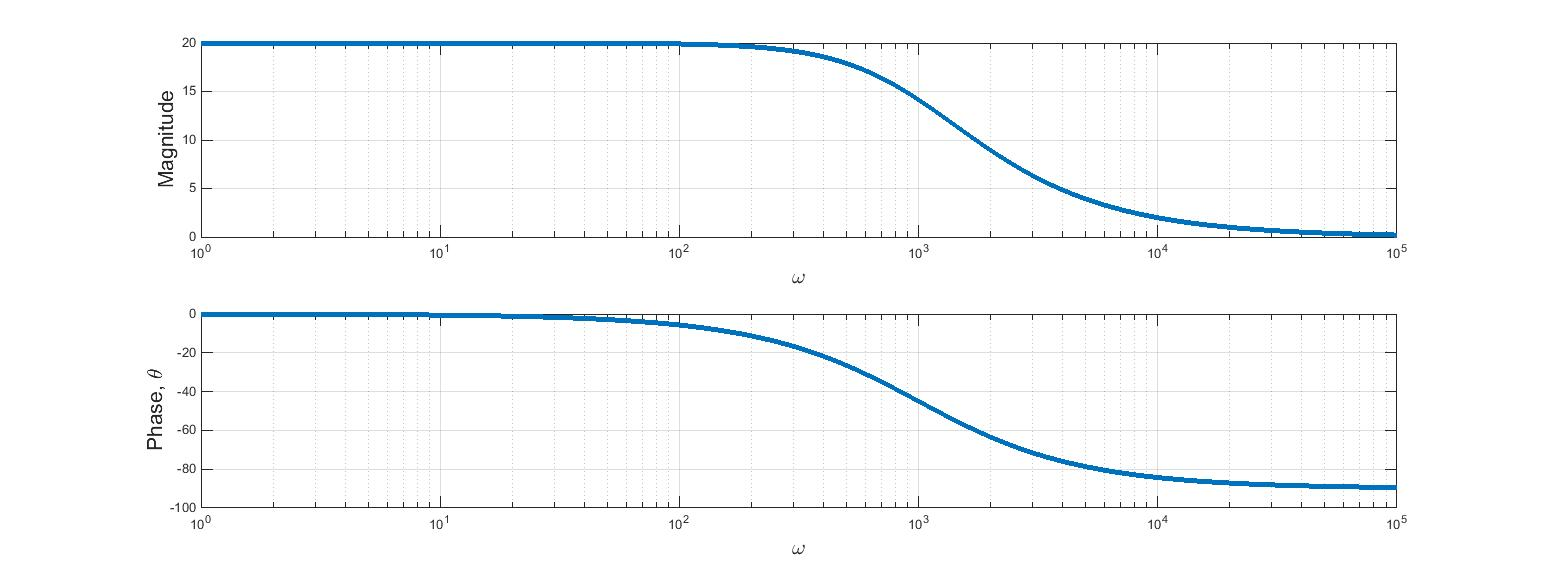
\includegraphics[width=1\textwidth]{Example1.jpg}
\end{figure}

Notice the gain has dropped to $14.14\ \  (0.707 \times 20)$ at $\omega = 1000$
}

\textbf{How would we build this filter?}  To build a first order LPF, we will start with one of the two circuits in Figure \ref{fig: LPF}. \textbf{Note:} Each of these circuits has a gain of 1; a gain greater than 1 requires an amplfication stage (think back to op amps).
\begin{figure} [h!]
\centering
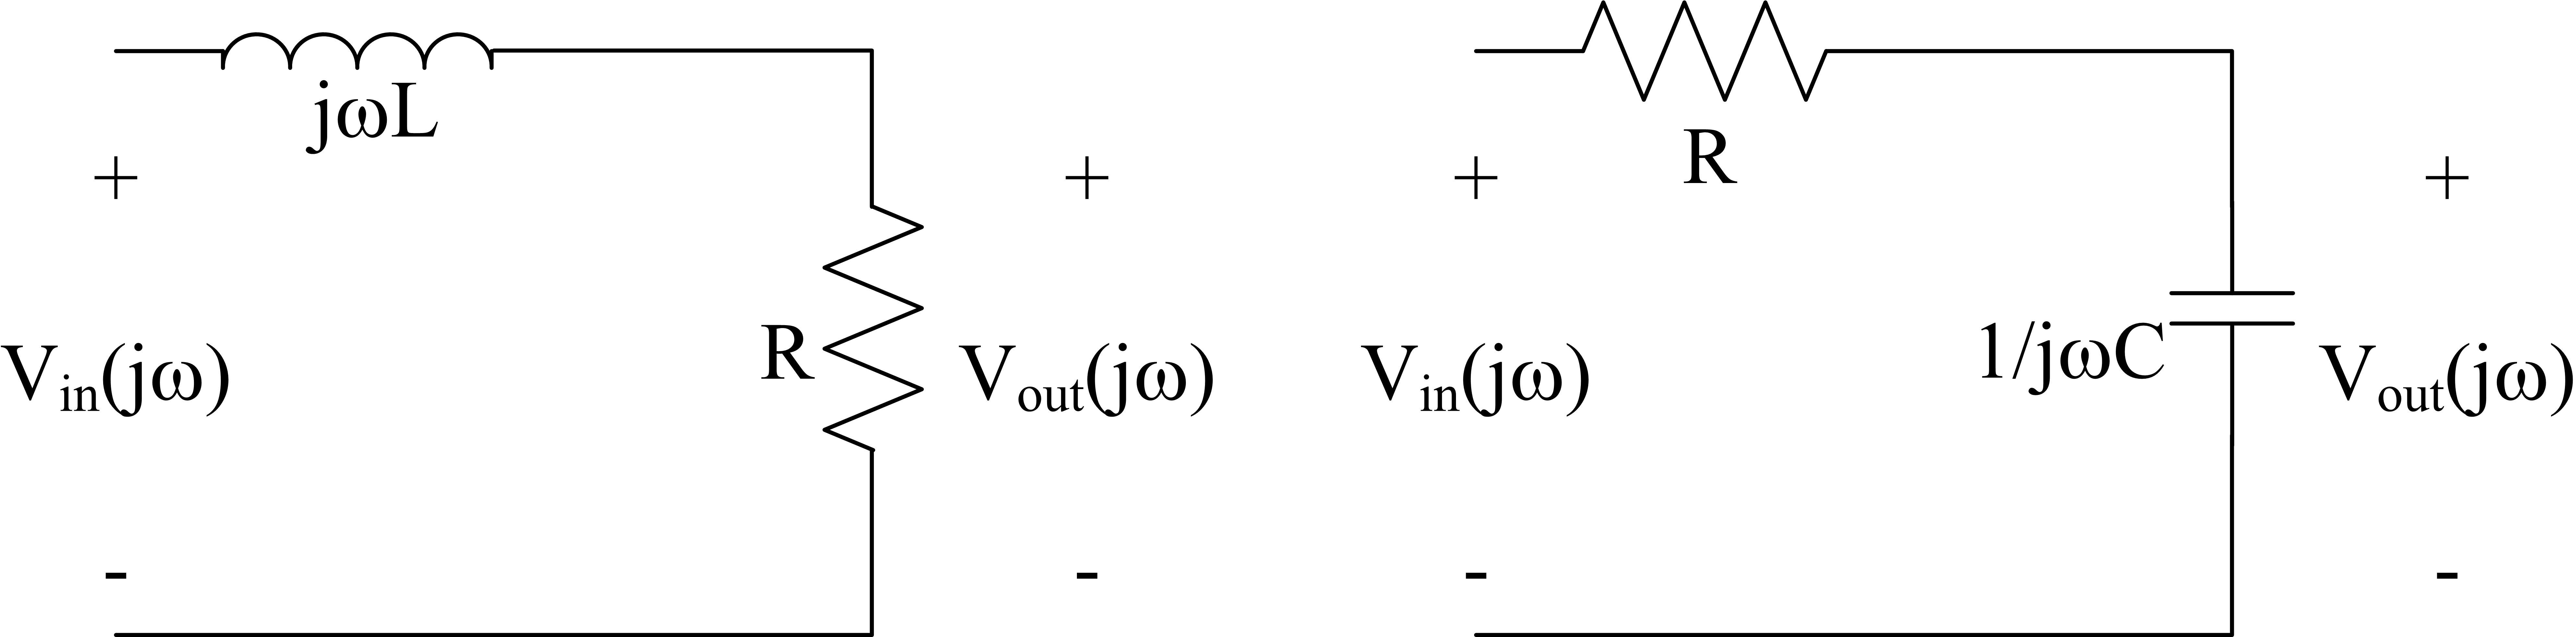
\includegraphics[width=0.65\textwidth]{LPF.jpg}
\caption{LPF circuits}
\label{fig: LPF}
\end{figure}

We can write transfer functions for these circuits:
\soln{1.5in}{
\[
H(j\omega) = \frac{\frac{R}{L}}{j\omega +\frac{R}{L}}
\]
\[
H(j\omega) = \frac{\frac{1}{RC}}{j\omega +\frac{1}{RC}}
\]
}

We could implement our example above by using a non-inverting op amp with $K=20$ and letting:
\soln{2in}{
\[
\frac{R}{L}=1000
\]
or
\[
\frac{1}{RC}=1000
\]
}

\newpage
\clearpage
\pagebreak

\subsection{High Pass Filters}
As the name implies, High Pass Filters (HPF) pass the high frequencies and block low frequency.  Another way to say this is that the {\em passband} includes frequencies from the cut-off frequency to infinity:
\soln{1in}{
\[
\omega_c<\omega_{pass}
\]
}

The {\em stopband} includes any frequency below the cutoff frequency.

The transfer function of a first order HPF is (memorize this form!):
\soln{1in}{
\[
H_{HPF}(j\omega) = K\frac{j\omega}{j\omega +\omega_c}
\]

Where $K$ is the gain and $\omega_c$ is the cut-off frequency
}

\textbf{Example 2} -- Plot the transfer function of
\[
H(j\omega) = \frac{j20\omega}{j\omega +1000}
\]
What is the {\em passband} gain? What is the cut-off frequency?
\soln{4in}{
First, we need to write the filter transfer function in standard form
\[
H(j\omega) = 20\frac{j\omega}{j\omega +1000}
\]

From here we can easily see that $K=20$ and $\omega_c=1000$
\begin{figure} [h!]
\centering
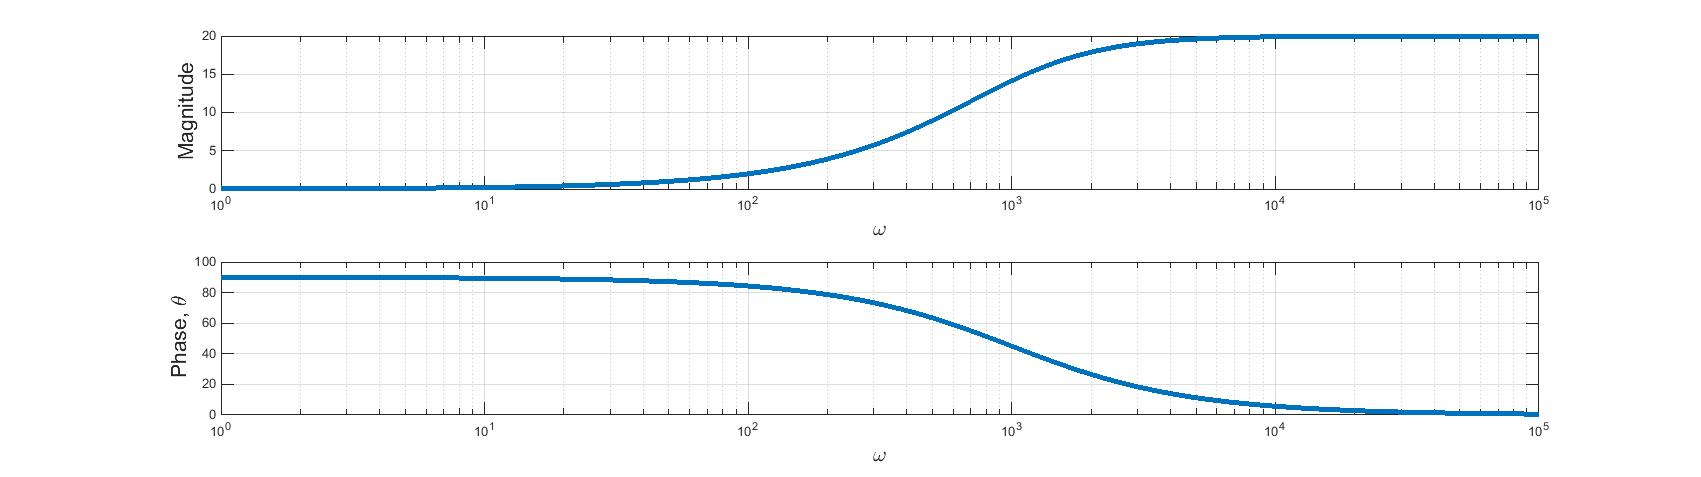
\includegraphics[width=1\textwidth]{Example2.jpg}
\end{figure}

Notice the gain has risen to $14.14\ \  (0.707 \times 20)$ at $\omega = 1000$
}

\newpage
\clearpage
\pagebreak

\textbf{How would we build this filter?}  To build a first order HPF, we will start with one of the two circuits in Figure \ref{fig: HPF}. \textbf{Note:} Each of these circuits has a gain of 1; a gain greater than 1 requires an amplfication stage (think back to op amps).
\begin{figure} [h!]
\centering
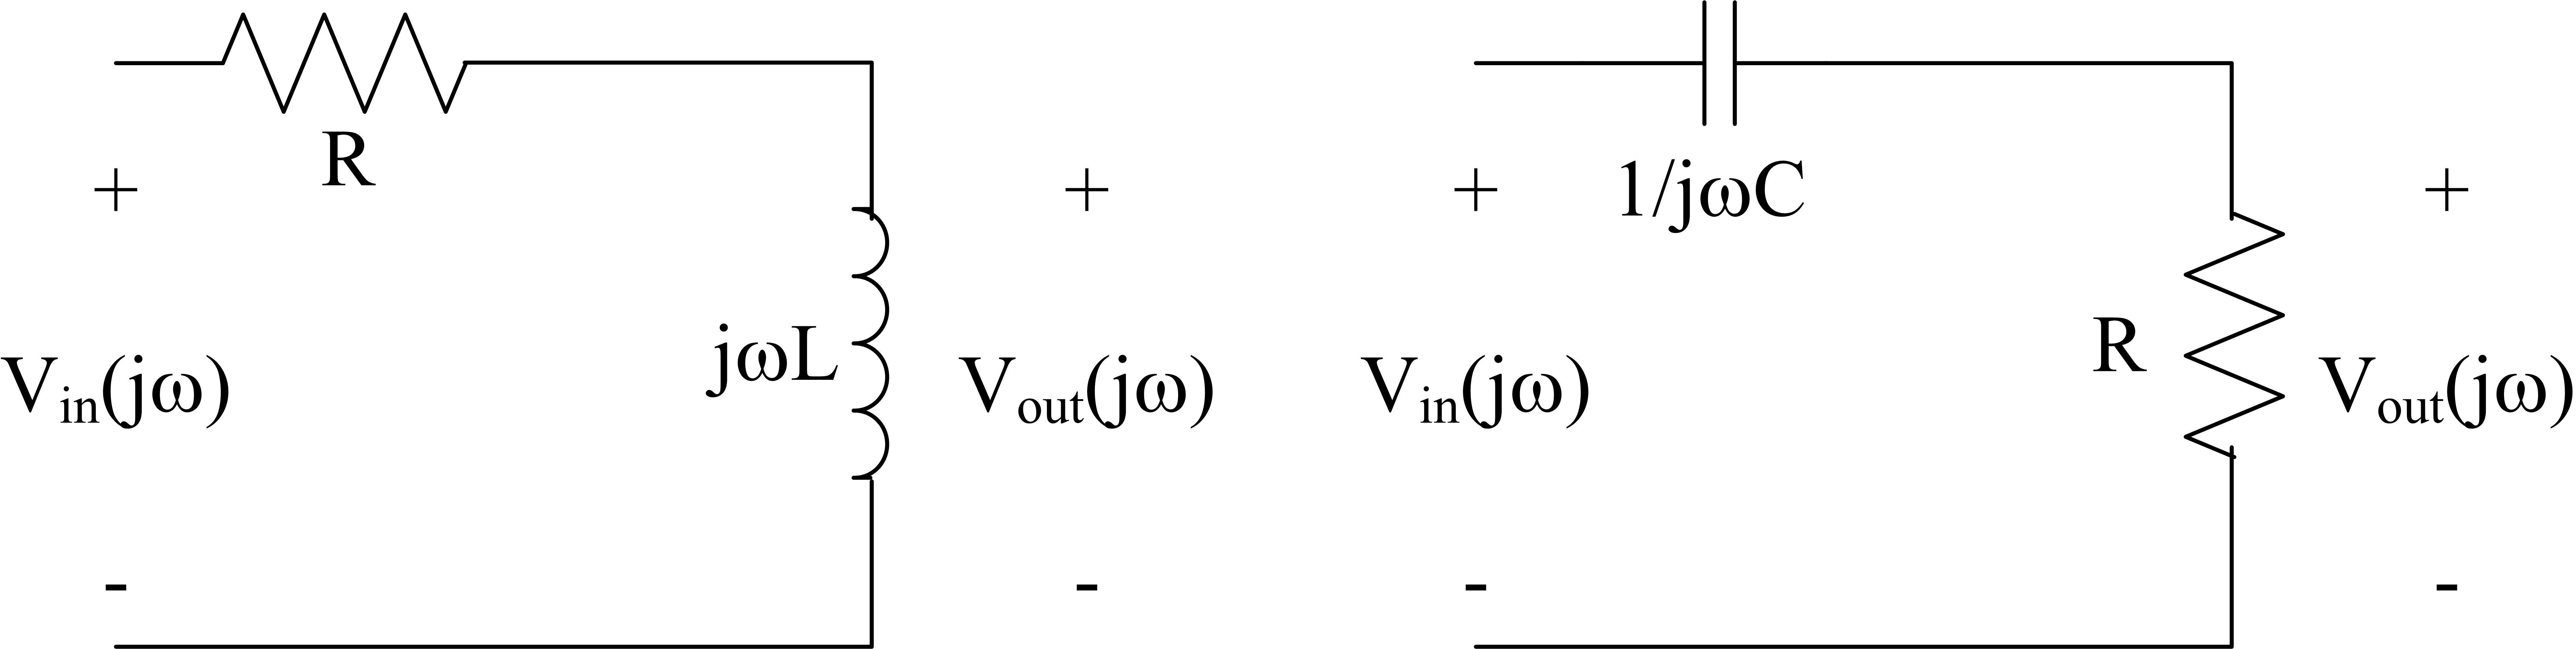
\includegraphics[width=0.65\textwidth]{HPF.jpg}
\caption{HPF circuits}
\label{fig: HPF}
\end{figure}

We can write transfer functions for these circuits:
\soln{2in}{
\[
H(j\omega) = \frac{j\omega}{j\omega +\frac{R}{L}}
\]
\[
H(j\omega) = \frac{j\omega}{j\omega +\frac{1}{RC}}
\]
}

We could implement our example above by using a non-inverting op amp with $K=20$ and letting:
\soln{2in}{
\[
\frac{R}{L}=1000
\]
or
\[
\frac{1}{RC}=1000
\]
}

\section{Cascaded Gain Stages with LPF and HPF}
We will not use class time to discuss this piece since it is relatively straight forward, but please read section 3.3 of the handout.  Take careful notice of the discussions on stage loading!

\newpage
\clearpage
\pagebreak

\section{Active Filters}
We can combine the gain stage and the filter stage by using active filters!  To do this, we will build our filter around an op amp.  We will show how to build filters using an inverting op amp and an $RC$ filter.  You can build filters with $RL$ filters and other op amp circuits as well.

\textbf{Example 3}  -- Two active filters are shown in Figures \ref{fig: ActiveLPF} and \ref{fig: ActiveHPF}; determine the transfer function of each filter and what type filter it is; also specify the gain.
\begin{figure} [h!]
\centering
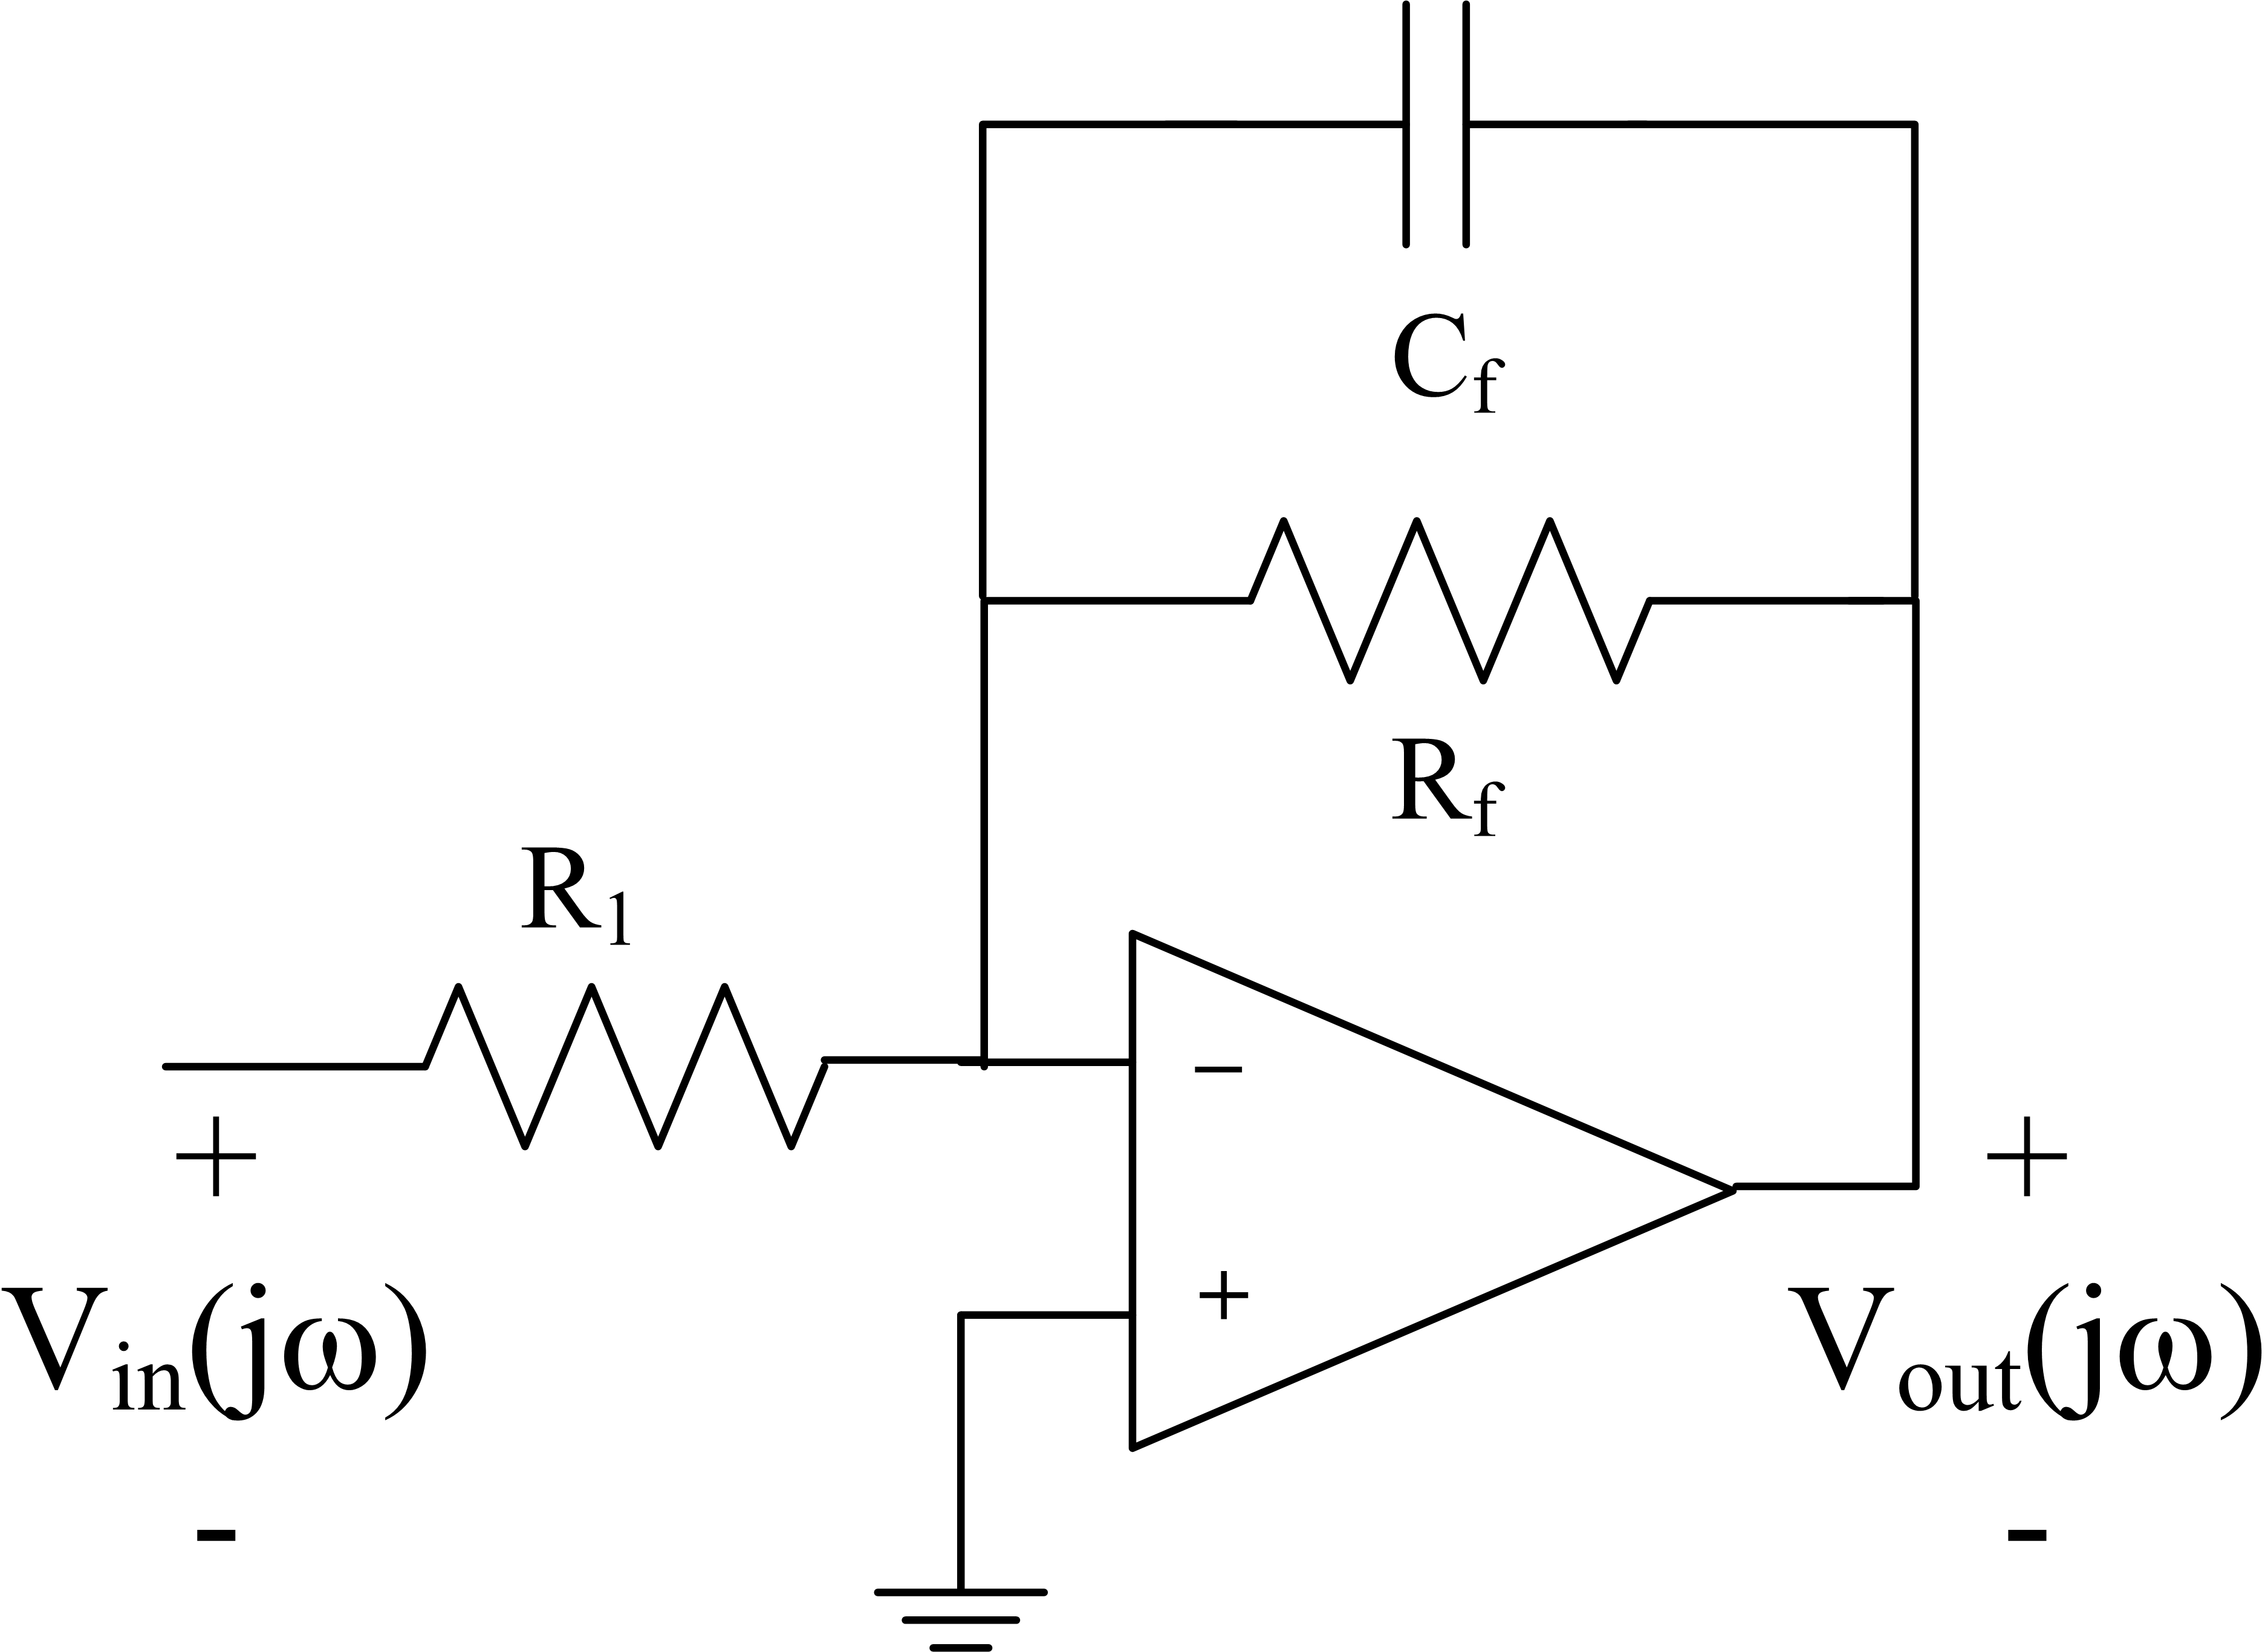
\includegraphics[width=0.6\textwidth]{ActiveLPF.jpg}
\caption{An active filter}
\label{fig: ActiveLPF}
\end{figure}
\begin{figure} [h!]
\centering
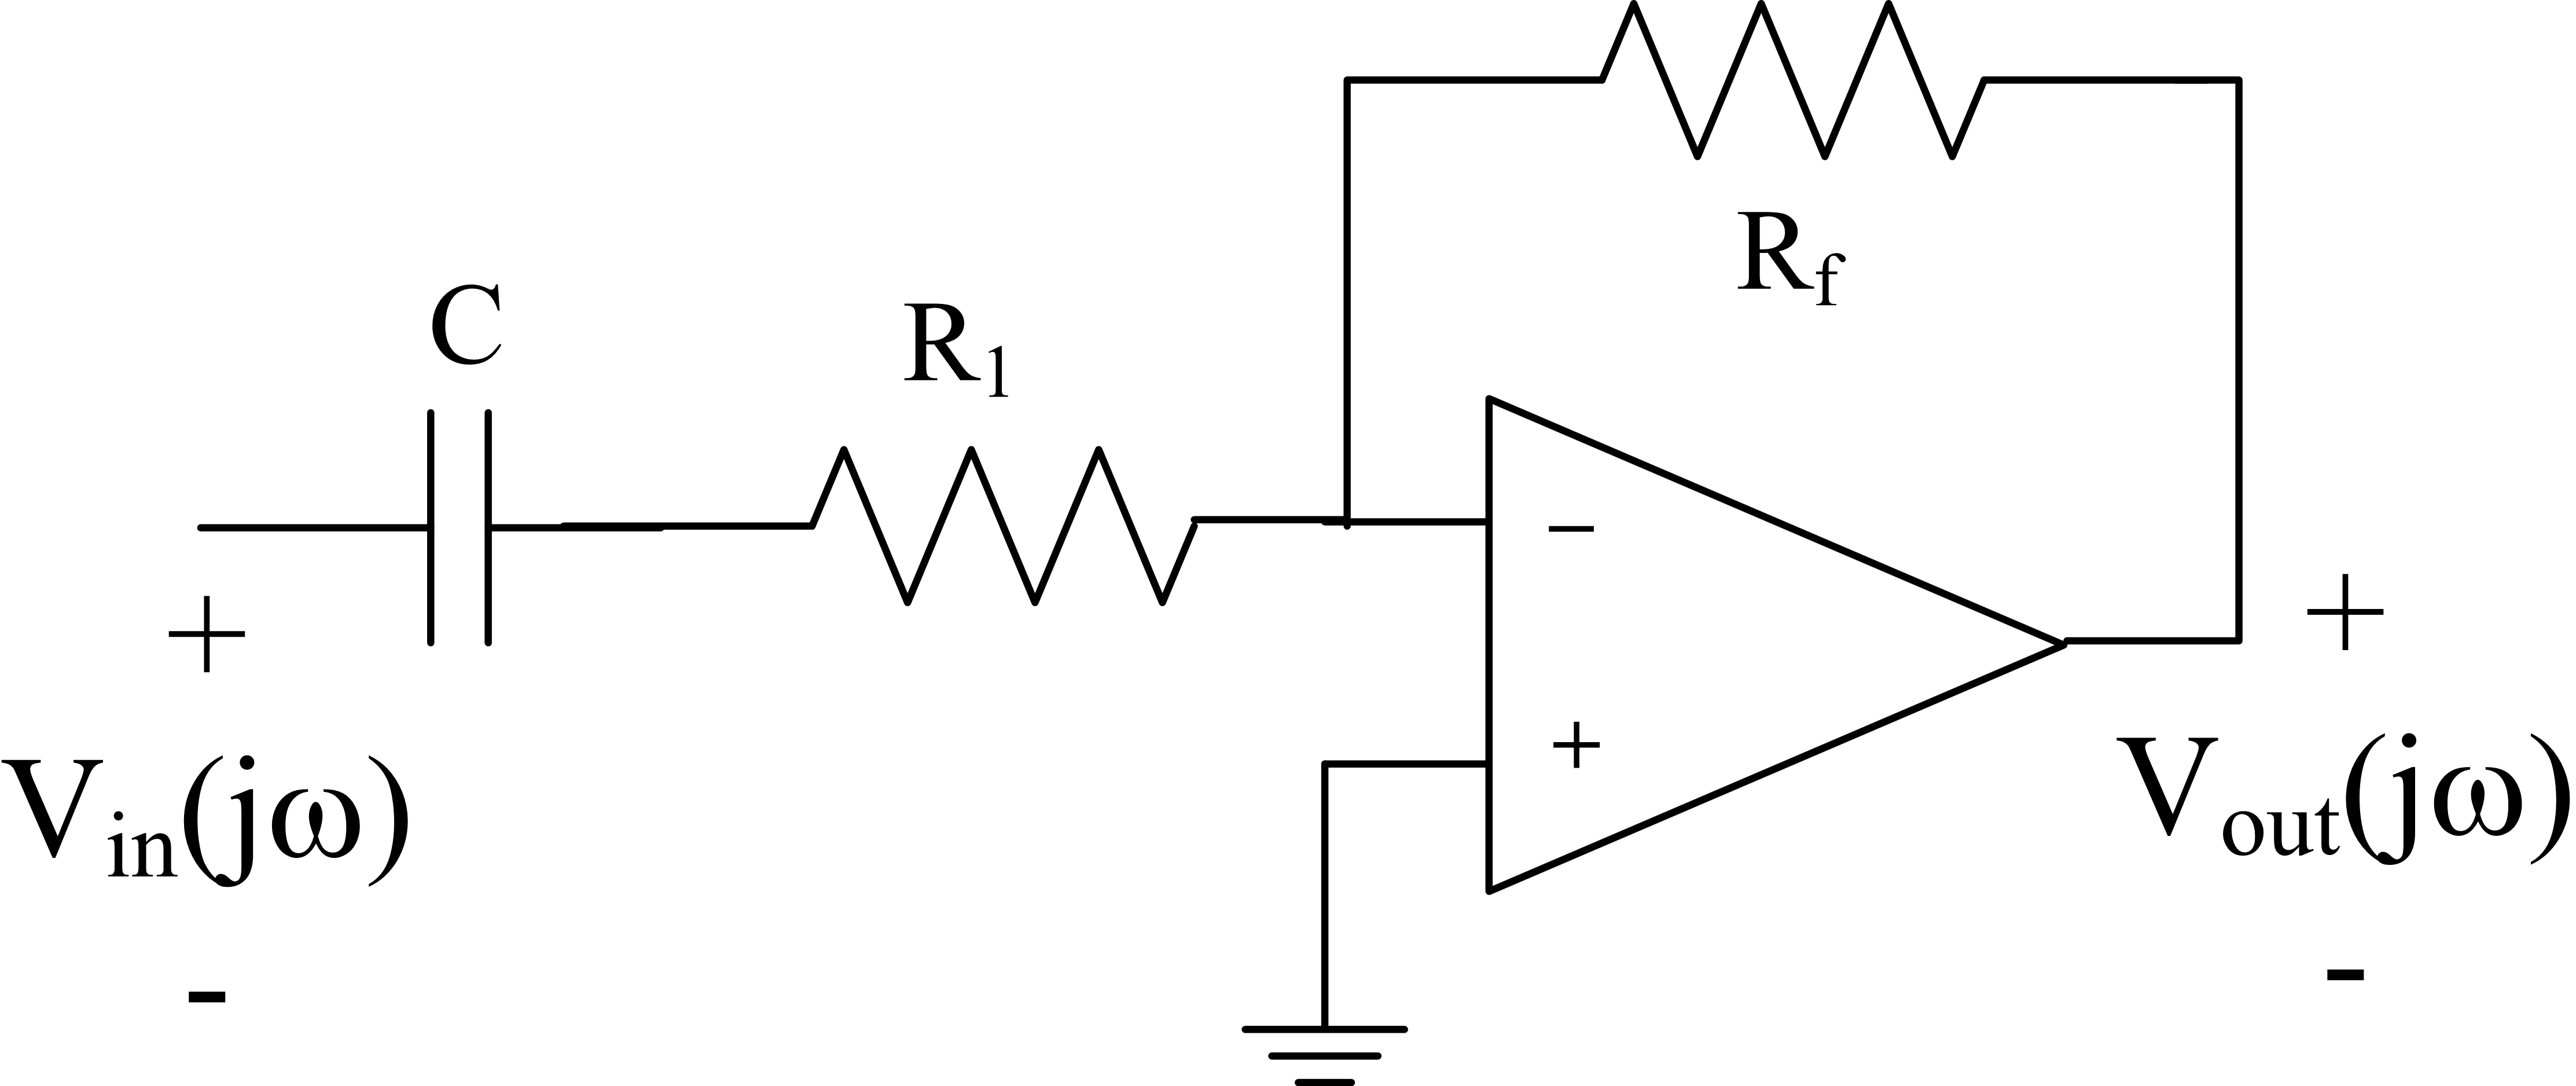
\includegraphics[width=0.7\textwidth]{ActiveHPF.jpg}
\caption{An active filter}
\label{fig: ActiveHPF}
\end{figure}

\soln{5in}{
\begin{figure} [h!]
\centering
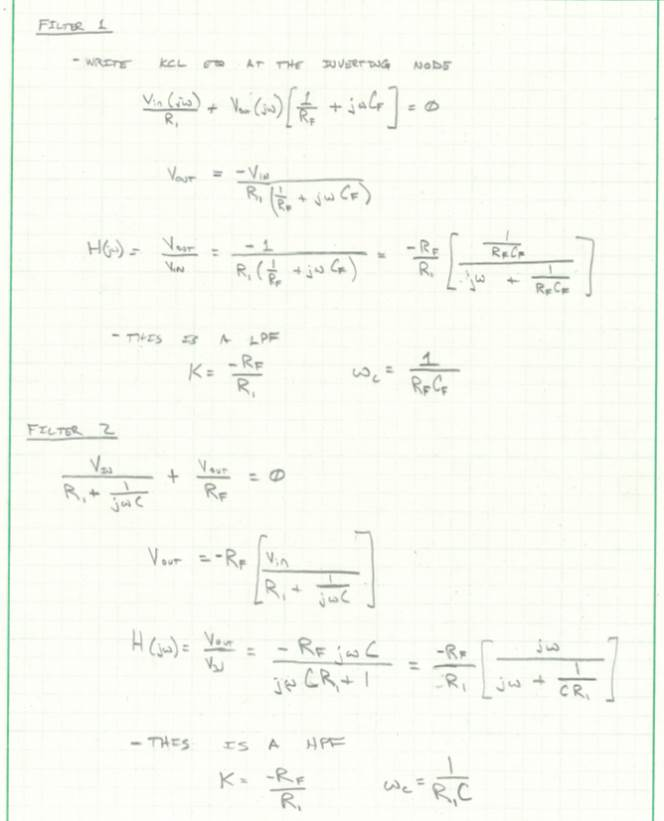
\includegraphics[width=1\textwidth]{Example3soln.jpg}
\end{figure}
}

\newpage
\clearpage
\pagebreak

\section{A Quick Primer on Decibels}
What is a decibel?  In short it is 10 times the  logarithm of a power ratio:
\soln{1in}{
\[
dB = 10\log \frac{P_{out}}{P_{in}}
\]
}

The only modification we need to make for our use is that we talk about {\em voltage gains}.  Recall that power is related to vootage squared.  This leads us to
\soln{1in}{
\[
dB =  10\log \left[\frac{V_{out}}{V_{in}}\right]^2 = 20\log \frac{V_{out}}{V_{in}}
\]
}

Most of our magnitude plots will be shown in dB.  Figure \ref{fig: dB} shows a magnitude plot of $\frac{200}{j\omega+50}$ in both absolute gain and in dB.
\begin{figure} [h!]
\centering
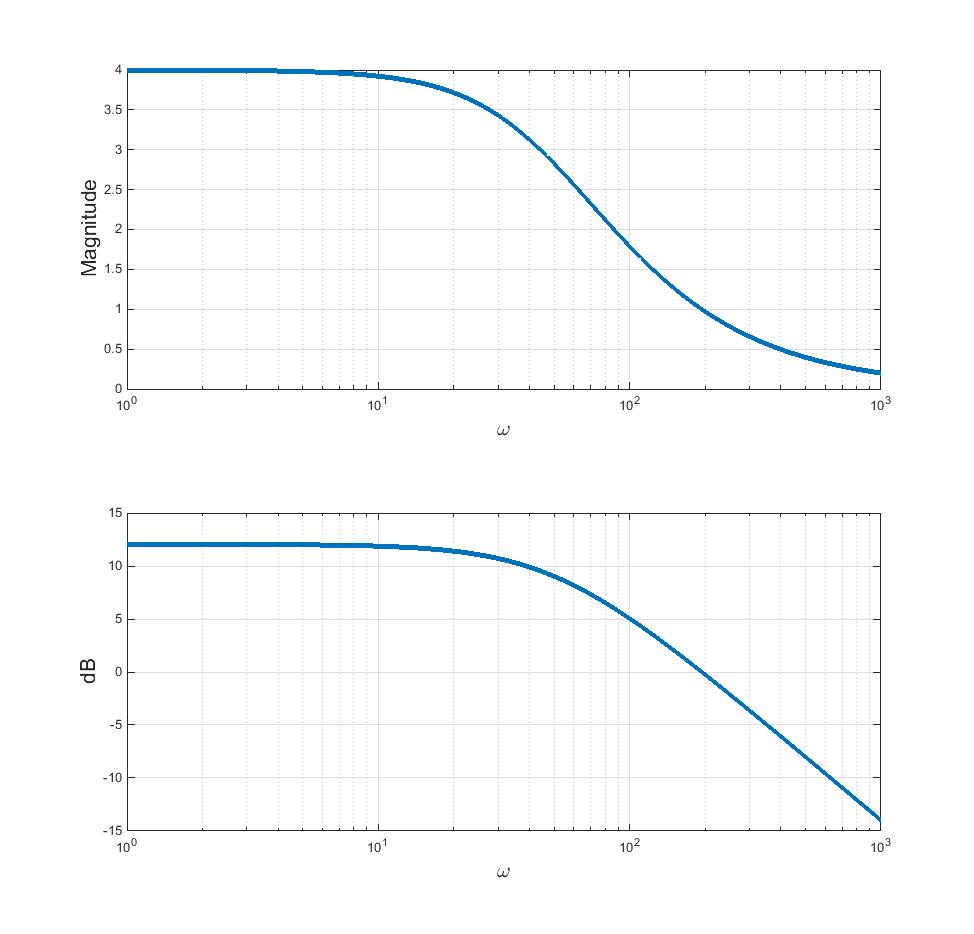
\includegraphics[width=0.7\textwidth]{dB.jpg}
\caption{Magnitude response in Gain and dB}
\label{fig: dB}
\end{figure}

\textbf{Note:}At the cut-off frequency, the gain is always $3\ dB$ below the maximum gain (or $-3\ dB$)

\newpage
\clearpage
\pagebreak

\newpage
\clearpage
\pagebreak

\newpage
\clearpage
\pagebreak

\newpage
\clearpage
\pagebreak

\newpage
\clearpage
\pagebreak

\newpage
\clearpage
\pagebreak

\end{document}


% Equation Array Example Code
%\begin
%{eqnarray}
%P_R &=& i_R^2R \nonumber \\
%P_R &=& (100\ mA)^2 \times 100\ \Omega \nonumber \\
%P_R &=& (100 \times 10^{-3}\ A)^2 \times 100\ \Omega \\
%P_R &=& 10000 \times 10^{-6}\ A^2  \times 100\ \Omega \nonumber \\
%P_R &=& 1\ W  \nonumber
%\end{eqnarray}

% Figure Example Code
%\begin{figure} [h!]
%\centering
%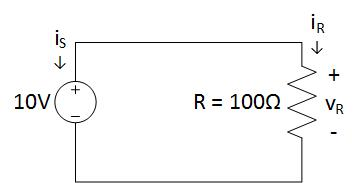
\includegraphics[width=0.5\textwidth]{OhmsLawExampleSolution.jpg}
%\caption{Ohm's Law example circuit}
%\label{fig: OhmsLawExampleSolution}
%\end{figure}

%Table Example Code
%\begin{table}[h]
%\centering
%\begin{tabular}{|l|c|c|}
%\hline
%Prefix & Abbreviation & Value \\
%\hline \hline
%Giga & $G$ & $10^9$ \\
%Mega & $M$ & $10^6$ \\
%Kilo & $k$ & $10^3$ \\
%\hline
%milli & $m$ & $10^{-3}$ \\
%micro & $\mu$ & $10^{-6}$ \\
%nano & $n$ & $10^{-9}$ \\
%pico & $p$ & $10^{-12}$ \\
%\hline
%\end{tabular}
%\caption{Engineering prefixes and values}
%\label{tab: Eng Prefixes}
%\end{table}
